% Kanizsa, alpha = 2
\begin{figure}
  \centering
    \makebox[\textwidth]{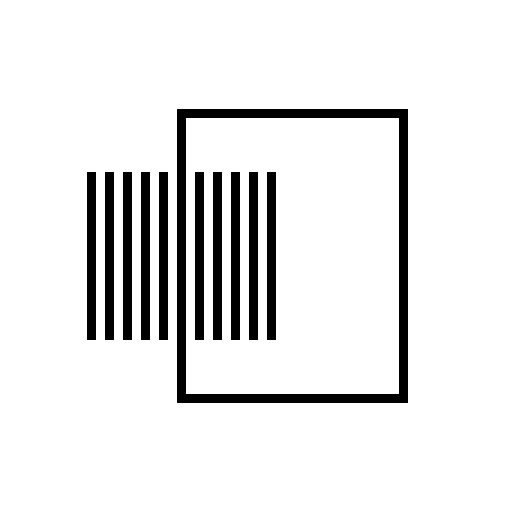
\includegraphics{./canny/kanizsa}} \\
  \caption{Original kanizsa image}
  \label{fig:kanizsa}
\end{figure}

\begin{figure}
  \centering
    \makebox[\textwidth]{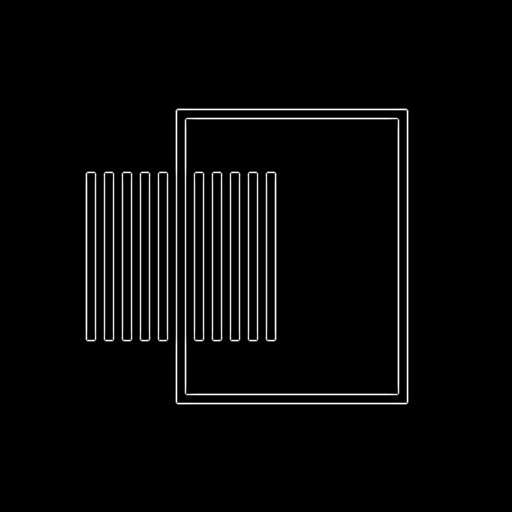
\includegraphics{./canny/kanizsa_LINF_a2_k11_k24}} \\
  \caption{kanizsa, Isotropic L-infinity norm. $\alpha$ = 2, K1 = 1, K2 = 4}
  \label{fig:kanizsa_LINF_a2_k11_k24}
\end{figure}

\begin{figure}
  \centering
    \makebox[\textwidth]{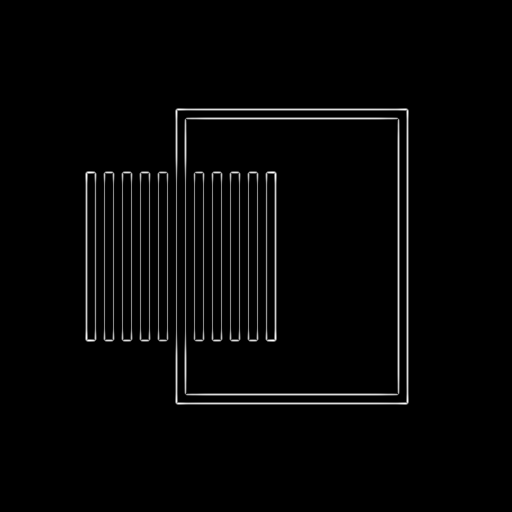
\includegraphics{./canny/kanizsa_L1_a2_k11_k24}} \\
  \caption{kanizsa, Isotropic L1 norm. $\alpha$ = 2, K1 = 1, K2 = 4}
  \label{fig:kanizsa_L1_a2_k11_k24}
\end{figure}

\begin{figure}
  \centering
    \makebox[\textwidth]{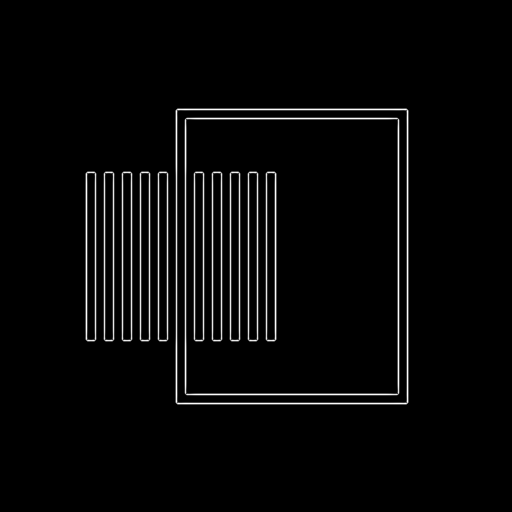
\includegraphics{./canny/kanizsa_L2_a2_k11_k24}} \\
  \caption{kanizsa, Isotropic L2 norm. $\alpha$ = 2, K1 = 1, K2 = 4}
  \label{fig:kanizsa_L2_a2_k11_k24}
\end{figure}

\begin{figure}
  \centering
    \makebox[\textwidth]{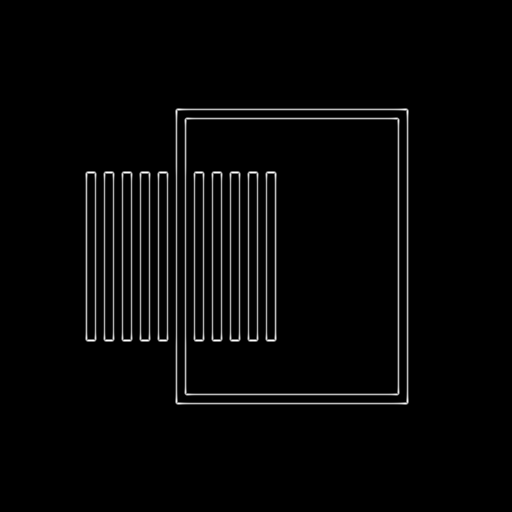
\includegraphics{./canny/kanizsa_ANISO_a2_k11_k24}} \\
  \caption{kanizsa, Anisotropic. $\alpha$ = 2, K1 = 1, K2 = 4}
  \label{fig:kanizsa_ANISO_a2_k11_k24}
\end{figure}